\documentclass[14pt]{article}
\usepackage[utf8]{inputenc}
\usepackage[russian]{babel}
\usepackage{geometry}
\usepackage{graphicx}
\usepackage{enumitem}
\usepackage{hyperref}
\usepackage{titlesec}
\usepackage{amsmath}
\usepackage{caption}
\usepackage{setspace}
\usepackage{indentfirst}
\usepackage[labelfont=normalfont]{caption}
\DeclareCaptionLabelSeparator{mysep}{~---~}
\captionsetup[figure]{name=Рисунок, labelsep=mysep, font=normalsize, justification=centering}


\geometry{
  a4paper,
  top=20mm,
  bottom=20mm,
  left=30mm,
  right=10mm
}
\titleformat{\section}
  {\normalfont\fontsize{14}{16}\selectfont} % обычный (не жирный) шрифт, 14 кегль, межстрочный интервал 16
  {\thesection}                             % номер раздела
  {1em}                                     % отступ между номером и заголовком
  {}                                        % без дополнительного кода
\setlength{\parindent}{1.25cm}
\setlist[itemize,1]{left=1.25cm, label=--, nosep}
\setlist[itemize,2]{left=0.25cm, label=•, nosep}

\setlist[enumerate,1]{left=1.25cm, nosep}
\setlist[enumerate,2]{left=0.25cm, nosep}




\sloppy

\title{Разработка клиент-серверного desktop-приложения для поддержки бизнес-процессов компании}
\author{}
\date{Москва, 2025}

\begin{document}
\onehalfspacing

\begin{center}
	МИНИСТЕРСТВО НАУКИ И ВЫСШЕГО ОБРАЗОВАНИЯ РОССИЙСКОЙ ФЕДЕРАЦИИ \\[0.2cm]
	ФЕДЕРАЛЬНОЕ ГОСУДАРСТВЕННОЕ АВТОНОМНОЕ ОБРАЗОВАТЕЛЬНОЕ УЧРЕЖДЕНИЕ ВЫСШЕГО ОБРАЗОВАНИЯ \\[0.2cm]
	\textbf{«МОСКОВСКИЙ ПОЛИТЕХНИЧЕСКИЙ УНИВЕРСИТЕТ» (МОСКОВСКИЙ ПОЛИТЕХ)} \\[1cm]
	Факультет информационных технологий \\[0.2cm]
	Кафедра «Инфокогнитивные технологии» \\[4 cm]

	\textbf{КУРСОВОЙ ПРОЕКТ} \\[0.2cm]
	на тему: \\
	\textit{«Веб-приложение для поиска партнеров по времени, месту и предпочтениям для занятий на уличных тренажерах»} \\[0.5cm]

	Направление подготовки 09.03.03 «Прикладная информатика» \\
	Профиль «Корпоративные информационные системы» \\
    
	 \vfill
     \hfill Выполнил: \\[0.2cm] 
     \hfill Студент группы 231-362 \\ 
     \hfill Ишмухаметов Даниль Ринатович \\ 
     \vfill
	Москва 2025
\end{center}

\newpage

\fontsize{14pt}{18pt}\selectfont

\section*{ Введение}
В условиях современного мегаполиса все больше людей стремятся вести здоровый образ жизни, используя доступные спортивные площадки.
Однако организация регулярных тренировок часто осложняется отсутствием надежных партнеров. Эта проблема особенно актуальна для Москвы,
где при высокой плотности населения многие испытывают трудности в поиске единомышленников для совместных занятий спортом.

Сложившаяся ситуация обусловлена несколькими факторами. Во-первых, социальные сети и приложения для знакомств, стриминговые платформы,
игры и подобные развлечения часто предлагают молодым людям более привлекательные альтернативы проведения свободного времени. Во-вторых,
недостаток мотивации играет огромную роль в отсутствии интереса к спортивным занятиям. В-третьих, социальные сети и приложения для знакомств не
адаптированы под специфику спортивных занятиях, не учитывают географическую близость пользователей к спортивным объектам.

Анализ современных решений показывает, что сервисы фокусируются преимущественно на организации групповых мероприятий, оставляя без внимания
потребность в индивидуальном подборе партнеров для регулярных занятий. Зарубежные аналоги часто оказываются неудобными для российских пользователей
из-за отсутствия информации о локальной инфраструктуре спортивных объектов.

Предлагаемый проект "Streetfit" разработан для решения этих проблем. Система реализует подбор партнеров на основе совместимости расписания,
возраста и географического расположения. Проект поможет решить проблемы пользователей, связанные с невозможностью оплатить фитнес в клубе,
предлагая выбрать один или несколько объектов, доступных для занятий спортом, на карте Москвы, а также проблему мотивации пользователей,
поскольку многие отмечают, что для начала регулярных занятий спортом им хотелось бы иметь товарища, чтобы добавить обязательности этим занятиям.

\newpage

\section*{1. Цель и задачи работы}
Цель работы — разработка веб-приложения для поиска спортивных партнеров на открытых площадках Москвы, обеспечивающего:
\begin{itemize}[noitemsep, topsep=0pt]
	\item автоматизированный подбор пользователей по географическому расположению и расписанию;
	\item безопасный обмен контактами при взаимной симпатии.
\end{itemize}
\indent Основные задачи:
\begin{enumerate}[noitemsep, topsep=0pt]
	\item Анализ существующих решений и выявление ключевых проблем поиска спортивных партнеров;
	\item Разработка инфологической, реляционной и физической моделей предметной области;
	\item Проектирование архитектуры приложения;
	\item Разработка клиентской части: интерфейс должен быть адаптивным и интерактивным;
	\item Создание серверной части для обработки запросов и хранения данных.
\end{enumerate}

Исходные данные: Набор данных «Тренажерный городок (воркаут)».

Средства разработки:
\begin{itemize}
	\item Клиентская часть:
	      \begin{enumerate}
		      \item React [1] – для создание пользовательских интерфейсов;
		      \item React Router [2] – для навигации между страницами;
		      \item JavaScript API Яндекс карт [3] – для размещения интерактивных карт;
		      \item Framer – для анимации интерфейса;
		      \item Lucide-React – набор иконок для использования их в виде React компонентов;
	      \end{enumerate}
	\item Серверная часть:
	      \begin{enumerate}
		      \item Node.js – среда выполнения JavaScript;
		      \item Express [4] – веб-фреймворк для создания обработчиков http запросов в разных
		            URL-адресах;
		      \item PrismaORM – объектно-реляционное отображение, для работы с базами данных с
		            помощью JavaScript;
		      \item Faker.js – наполнение базы данных тестовыми данными;
		      \item Nodemon – для автоматического перезапуска сервере при разработке;
		      \item Jsonwebtoken – для создания и валидации JWT [5];
		      \item Bcrypt – для хэширования и проверки паролей
	      \end{enumerate}
	\item База данных – PostgreSQL
\end{itemize}
\newpage
\section*{ Проектирование приложения}
При проектировании приложения был определен следующий минимальный функционал: регистрация и авторизация пользователей, создание пользовательских карточек, содержащих информацию об удобном расписании пользователя, предполагаемых местах тренировок, а также возраст пользователя и его контактные данные.
Для реализации описанного функционала были спроектированы следующие сущности:
\begin{itemize}
	\link Пользователь – содержит необходимые поля для реализации авторизации и аутентификации (email, пароль), контактные данные и возраст;
	\link Расписание – содержит информацию, в какой день и в какое время пользователь готов заниматься;
	\link Локация – содержит геолокацию спортивного объекта (долготу и широту);
	\link Спортивный объект – содержит информацию, предлагаемую открытым набором данных, а также локацию;
	\link Карточка пользователя – содержит информацию о расписании пользователя и спортивные объекты, где пользователь хочет заниматься;
	\link Лайк и дизлайк – содержат информацию, какой пользователь какую карточку оценил, и в какое время.
\end{itemize}
На основе описанный сущностей была спроектированы инфологическая, реляционная и физическая модель предметной области.

\begin{figure}[H!]
	\centering
	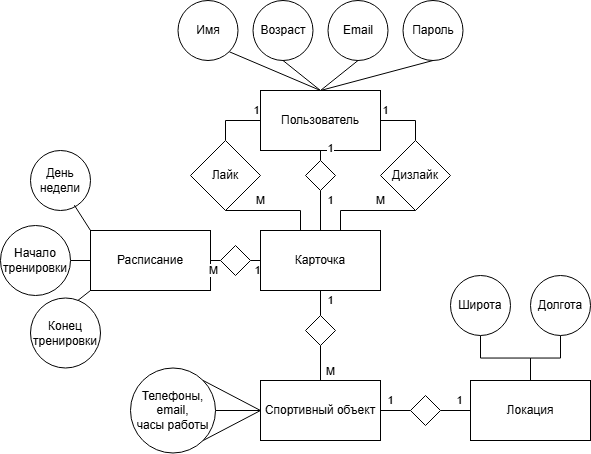
\includegraphics[width=0.8\textwidth]{fig1.png}
	\caption{Инфологическая модель предметной области}
\end{figure}

\begin{figure}[H!]
	\centering
	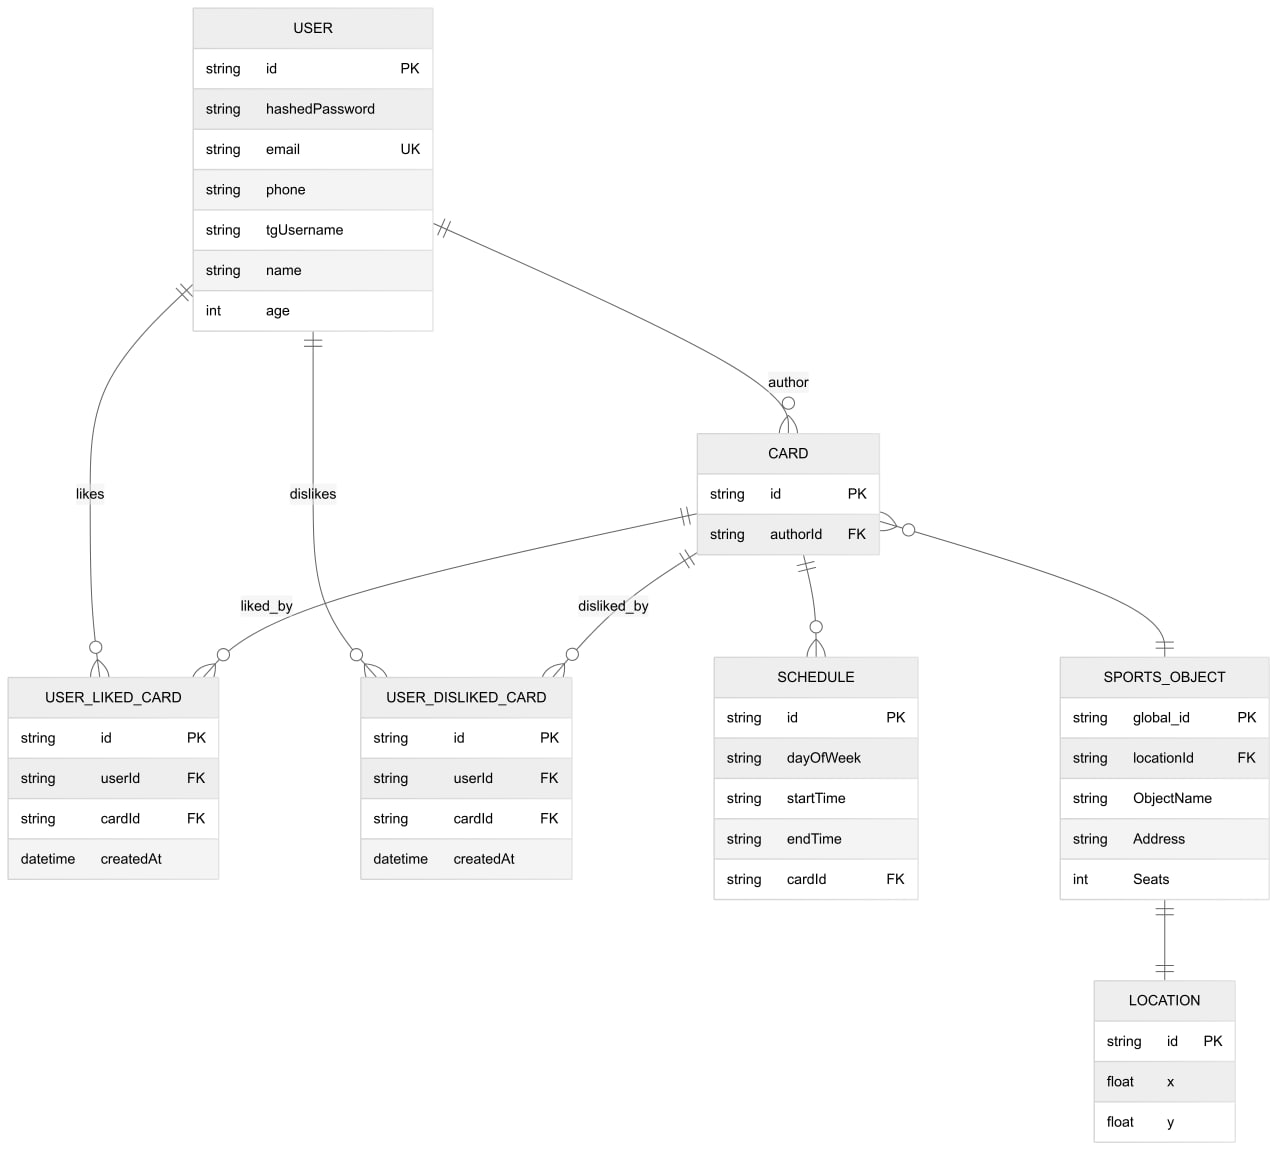
\includegraphics[width=0.8\textwidth]{fig2.png}
	\caption{Реляционная модель предметной области, нотация Мартина}
\end{figure}

\begin{figure}[H!]
	\centering
	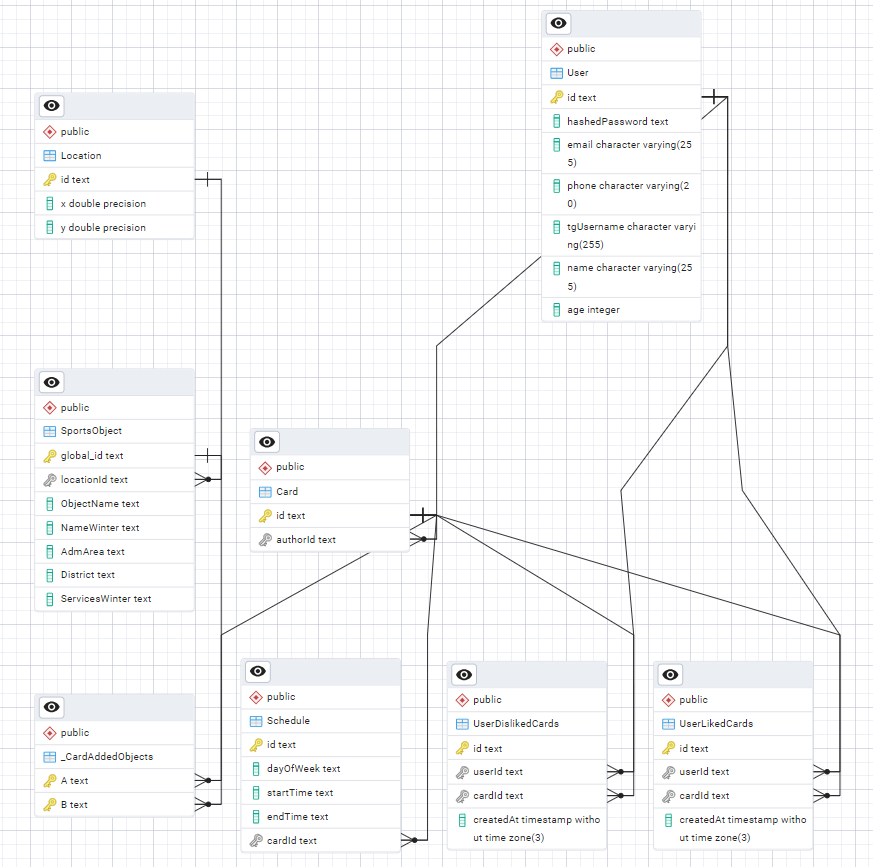
\includegraphics[width=0.8\textwidth]{fig3.png}
	\caption{Физическая модель предметной области}
\end{figure}

Пользовательский интерфейс имеет единообразную карточную структуру.
В левой части приложения располагается адаптивный сайдбар для навигации по приложению, выхода из
аккаунта пользователя и переключения цветовой темы. В зависимости от ширины экрана он меняет свое местоположение,
надписи скрываются, чтобы не занимать лишнее место на странице и не отвлекать пользователя от просмотра контента (карточек других пользователей).

В основной области приложения располагаются карточки пользователей, содержащие информацию об удаленности
от пользователя выбранных другими пользователями спортивных объектов, имя и возраст пользователя, а также совпадающие расписания.
Карточки адаптивно изменяют свой размер в зависимости от ширины экрана, изменяется количество столбцов. При нажатии пользователем на данные
о местоположении объектов в карточке разворачивается карта, на которой отмечены спортивные объекты, которые выбрал пользователь.
Кроме того, выделены дни, в которые расписания пользователей перекрываются. Добавлена кнопка «Показать все дни», чтобы пользователь мог ознакомиться,
в какие еще дни готов заниматься потенциальный новый товарищ.

Приложение логически разделено на следующие страницы:
\begin{itemize}
	\item Главная – пользователь смотрит карточки потенциальных товарищей, ставит лайки/дизлайки, после чего карточки пропадают из ранжированного списка;
	\item Лайки – пользователь видит карточки пользователей, которые поставили лайк карточке пользователя;
	\item Контакты – пользователь видит карточки пользователей, с которыми произошел мэтч (взаимный лайк), уже с контактной информацией для связи;
	\item Профиль – пользователь видит свои данные и может их отредактировать в любой момент;
	\item Авторизация – содержит карточки с формой авторизации, поля валидируются;
	\item Регистрация – содержит карточки с описанием сервиса и формой регистрации, поля валидируются;
	\item Onboarding – после первой авторизации на сайте пользователь заполнет свою
	      «карточку» с именем и возрастом, выбирая дни и время тренировок, места занятий.
\end{itemize}
Сервер, в свою очередь, обрабатывает http запросы, отправляемые из браузера пользователя. Для этого разработаны соответствующие контроллеры:
\begin{itemize}
	\item Контроллер авторизации, содержащий всю логику для регистрации и авторизации пользователя;
	\item Контроллер лайков, содержащий методы для создания записи о том, какую карточку оценил пользователь;
	\item Контроллер пользователя, содержащий логику, обеспечивающую утилитарную функцию приложения: персонолизированное предложение карточек других пользователей, просмотр мэтчей и лайков.
\end{itemize}
Для получения и записи данных в базу реализован слой доступа к данным в виде соответствующих репозиториев.
\newpage

\section*{Реализация приложения}

Для реализации приложения были определены основные маршруты и их функциональное назначение.

Регистрация и авторизация пользователей реализована с помощью форм, кнопка отправки вызывает валидацию формы,
пользователю показываются ошибки, если такие обнаружены. Текущие значения и ошибки сохраняются в React состояния.
Если ошибок не обнаружено, отправляется POST запрос на сервер, где происходит регистрация/аутентификация пользователя, в результате
чего тот получает сообщение об ошибке, например, если пользователь с введеным email уже зарегистрирован или введен неверный пароль.
В том случае, если данные введены верно, в случае регистрации – пароль хэшируется и сохраняется в базу данных, в случае авторизации –
пароль сравнивается с хэшем, хранящемся в базе данных, если все прошло успешно, в браузер возвращается ответ со статусом 200 (Success),
устанавливается Cookie «access$_$token» с атрибутом httpOnly для предотвращения доступа к кукам из JavaScript, устанавливается время жизни Cookie,
по истечении которого, пользователю предлагается авторизоваться заново.

\begin{figure}[H!]
	\centering
	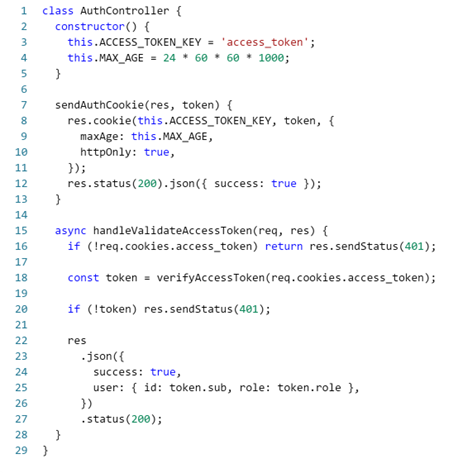
\includegraphics[width=0.8\textwidth]{fig4.png}
	\caption{Установка токена в Cookie и его валидация}
\end{figure}

В теле токена содержится информация об уникальном идентификаторе пользователя. Cookie «access$_$token»
отправляется с каждым запросом на сервер, что позволяет по наличию и проверке подписи токена, определять,
какой пользователь пытается получить/отправить данные. Такой подход позволяет не хранить сессию пользователя в базе данных.

При попытке пользователя посетить страницу, которая не должна быть доступна неавторизованным личностям, на сервер
отправляется запрос на проверку авторизации, и если проверка не будет пройдена, пользователь будет перенаправлен на страницу
авторизации, в случае успеха – на защищенную страницу.

\begin{figure}[H!]
	\centering
	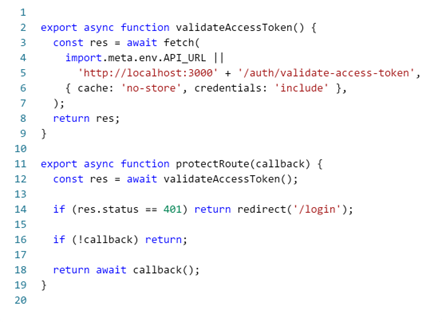
\includegraphics[width=0.8\textwidth]{fig5.png}
	\caption{Рисунок 5 — Валидация токена перед клиентской навигацией}
\end{figure}

Запрос, отправленный на сервер, прежде чем его обработает соответствующий метод контроллера проходит несколько
промежуточных модулей (middleware). «ctxMiddleware» проверяет наличие токена в Cookies, если таковой имеется, после
чего записывает пользовательский идентификатор в контекст, который доступен следующим обработчикам. Защищенные маршруты
обрабатывает «withAuthMiddleware», который в свою очередь проверяет уже контекст, описанный на предыдущем шаге, если контекст
не задан, возвращается ответ со статусом 401 (Unauthorized), после чего пользователя перенаправляет на страницу авторизации.
«errorMiddleware» содержит обработчик ошибок, в теле которого вызывается уже соответствующий метод контроллера, и в случае ошибки
логирует ошибку и возвращает ответ со статусом 500 (Internal Server Error).

\begin{figure}[H!]
	\centering
	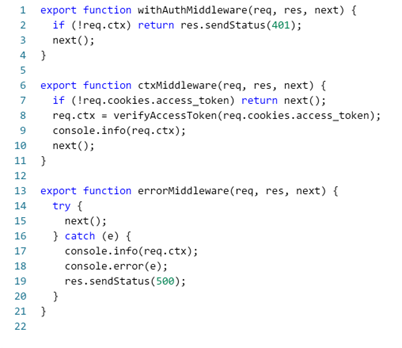
\includegraphics[width=0.8\textwidth]{fig6.png}
	\caption{Middleware}
\end{figure}

После регистрации пользователя при его попытке попасть к основным страницам происходит проверка, создал ли он карточку,
и если нет – происходит перенаправление на страницу onboarding’a.

Страница Onboarding реализована в виде листающихся карточек, на каждой из который предлагается заполнить имя, возраст,
расписание и указать места занятий. Номер текущей карточки записывается в состояние компонента. При попытке создания
карточки (нажатия кнопки подтверждения) происходит валидация всех полей, все ошибки записываются в состояние и карточки
листаются к первой, где возникла ошибка. После исправления, пользователь создает свою карточку и видит основной контент приложения.

В основной части приложения есть общий контейнер, внутри которого реализован адаптивный сайдбар для навигации по страницам сайта.
С помощью CSS медиа-запросов он изменяет свое положение в соответствие с размером viewport. На больших экранах он отображается
с левой стороны, рядом с контентом, на мобильных и маленьких экранах – подписи кнопок скрываются, а сайдбар закрепляется в нижней части страницы.
\begin{figure}[H!]
	\centering
	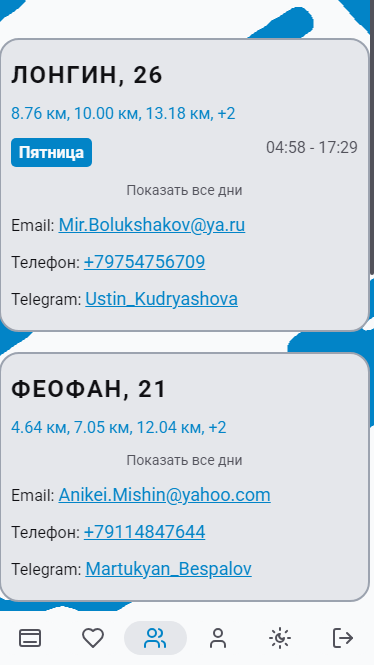
\includegraphics[width=0.8\textwidth]{fig7.png}
	\caption{Мобильная версия}
\end{figure} –

React позволяет переиспользовать компоненты, что значительно ускоряет
разработку и уменьшает кодовую базу приложения. Для всех карточек был написан
компонент Card, который уже был переиспользован для создания карточек
пользователей и карточек авторизации и регистрации.

Карточки пользователей используют обработчики пользовательских жестов и анимированы
с помощью framer. При «свайпах» вправо/влево пользователь лайкает/дизлайкает карточку
соответственно, и на сервер отправляется соответствующий запрос, содержащий идентификатор карточки.

Переключение темы реализовано добавлением CSS класса на корневой элемент html документа.
Использованы CSS переменные для указания цветов компонентов, которые переопределяются в CSS классе
dark. Создан React контекст, который позволяет получить текущую тему и функцию переключения темы в
дочернем компоненте любой вложенности (используется в компоненте сайдбара для переключения темы нажатием кнопки).

Для подключения и обращения к базе данных использована PrismaORM, предоставляющая возможность писать объектные
запросы, а не чистые SQL - запросы, что ускоряет разработку, а также позволяет избегать SQL – инъекций, повышая
тем самым отказоустойчивость и безопасность системы.

URL базы данных и секрет для подписи токенов выделены в переменные среды в
отдельном файле «.env», чтобы отделить конфигурационные данные от основной
логики приложения.

Была спроектирована и реализована система ранжирования пользовательских карточек. Каждая карточка оценивается следующим образом:
\begin{enumerate}
	\item Прежде всего считается разница в возрасте двух пользователей;
	\item Считаются и сортируются расстояния до спортивных объектов, которые выбрал другой пользователь;
	\item Считаются и сортируются совпадения расписаний (в минутах);
\end{enumerate}
Лучшие показатели расстояний и расписаний, разница в возрасте нормируются, умножаются на веса (0.5, 0.5 и 0.3 соответственно), после чего складываются для получения оценки карточки.

Такой алгоритм позволяет показывать пользователю наиболее релевантные карточки других пользователей, чтобы ускорить поиск товарища для занятий спортом.

Для заполнения данными с набора данных, написан скрипт, который парсит выгрузку набора данных в формате .csv и делает записи в базу данных.
Аналогично, для демонстрации функционала приложения написан скрипт, генерирующий данные, имитирующие данные реальных пользователей.

Оптимизация зависимостей клиентской части и сборка проекта осуществляется Vite,
который также предлаегает режим разработки с удобным автоматическим обновлением страниц при внесении изменений в код.

Для разработки серверной части в среде выполнения Node,
используется nodemon, который отслеживает изменения в директории и перезапускает
сервер, предлагая возможность удобной разработки без бесконечных ручных перезапусков.

Основные сценарии использования приложения

Примером использованиия приложения пользователем будет следующая последовательность.
Открытие сайта встретит пользователя формой авторизации с предложением создать аккаунт.

\begin{figure}[H!]
	\centering
	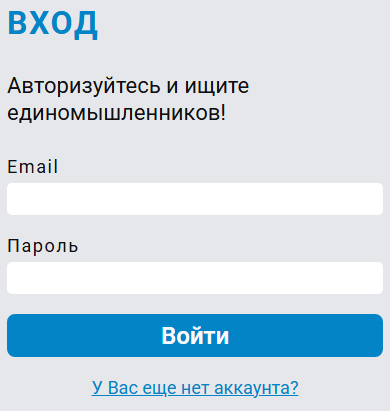
\includegraphics[width=0.8\textwidth]{fig8.png}
	\caption{Форма авторизации}
\end{figure}

Пользователь, у которого еще нет аккаунта перейдет на страницу регистрации.

\begin{figure}[H!]
	\centering
	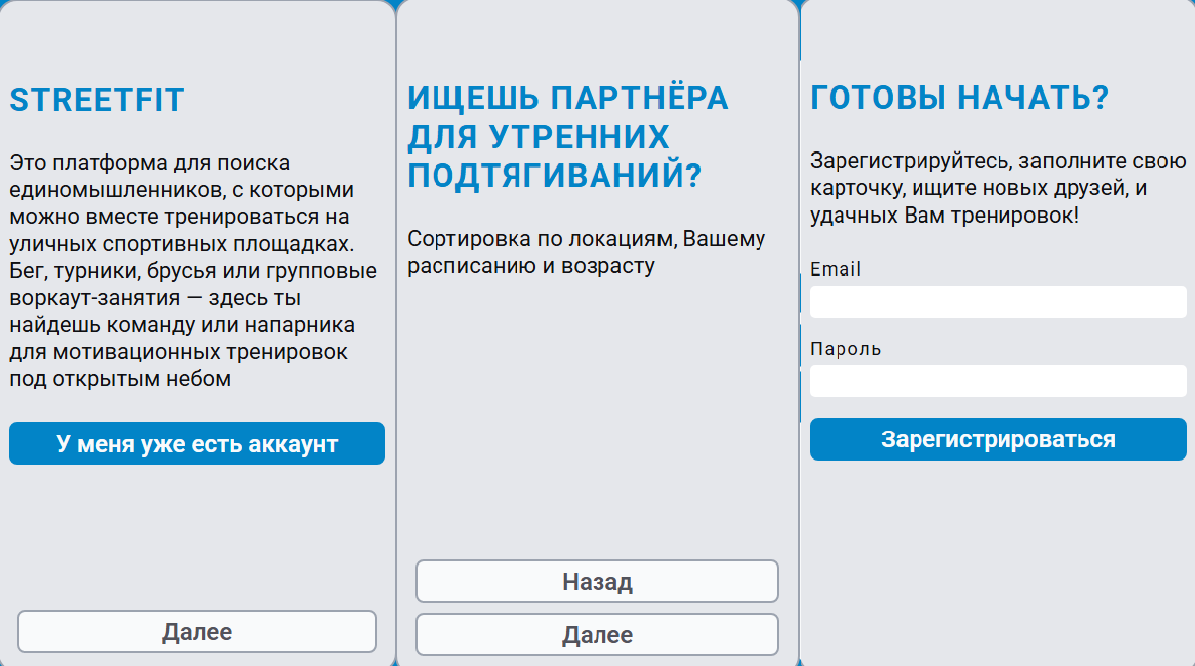
\includegraphics[width=0.8\textwidth]{fig9.png}
	\caption{Карточки на странице регистрации}
\end{figure}

После регистрации пользователю будет предложено заполнить его карточку, которую будут видеть остальные.

\begin{figure}[H!]
	\centering
	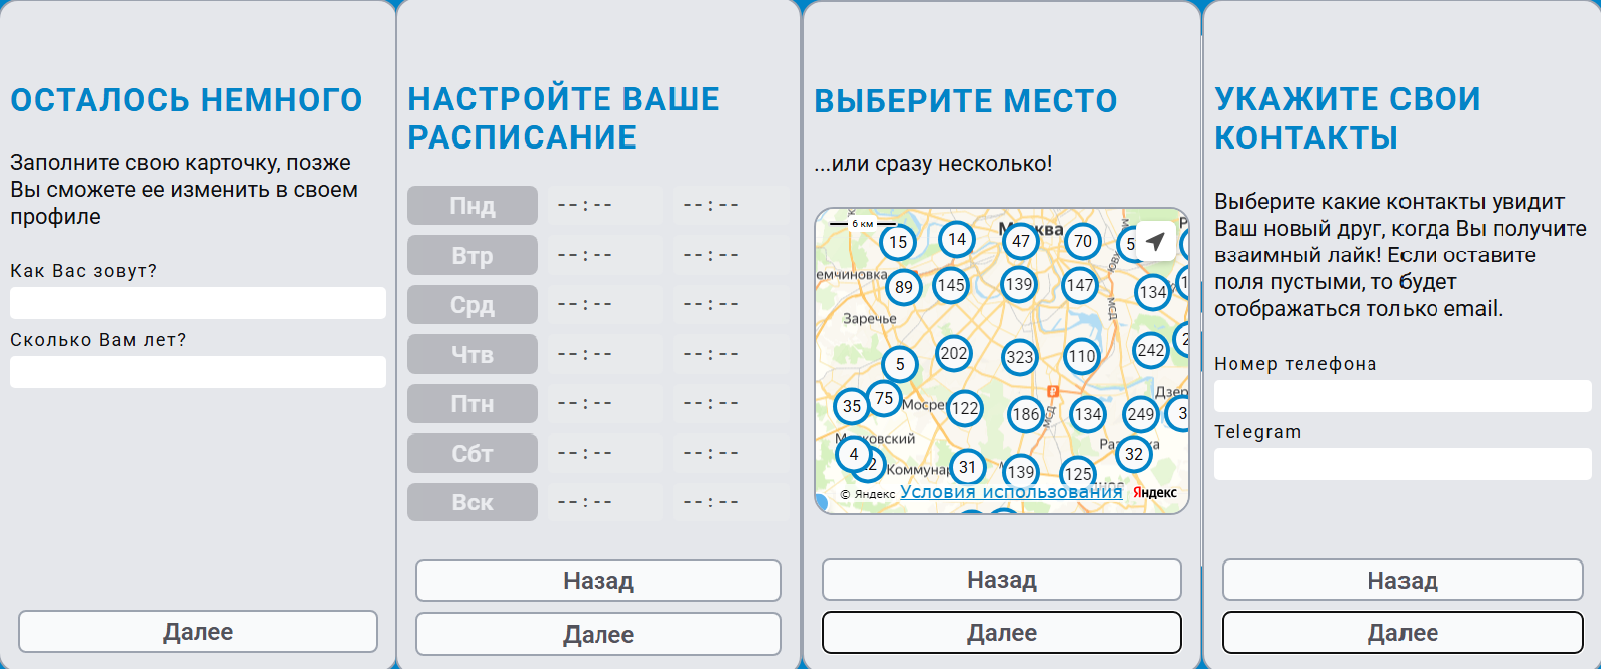
\includegraphics[width=0.8\textwidth]{fig10.png}
	\caption{Форма для заполнения карточки пользователя}
\end{figure}

После заполнения всех форм пользователь сможет видеть и оценивать карточки других пользователей.

\begin{figure}[H!]
	\centering
	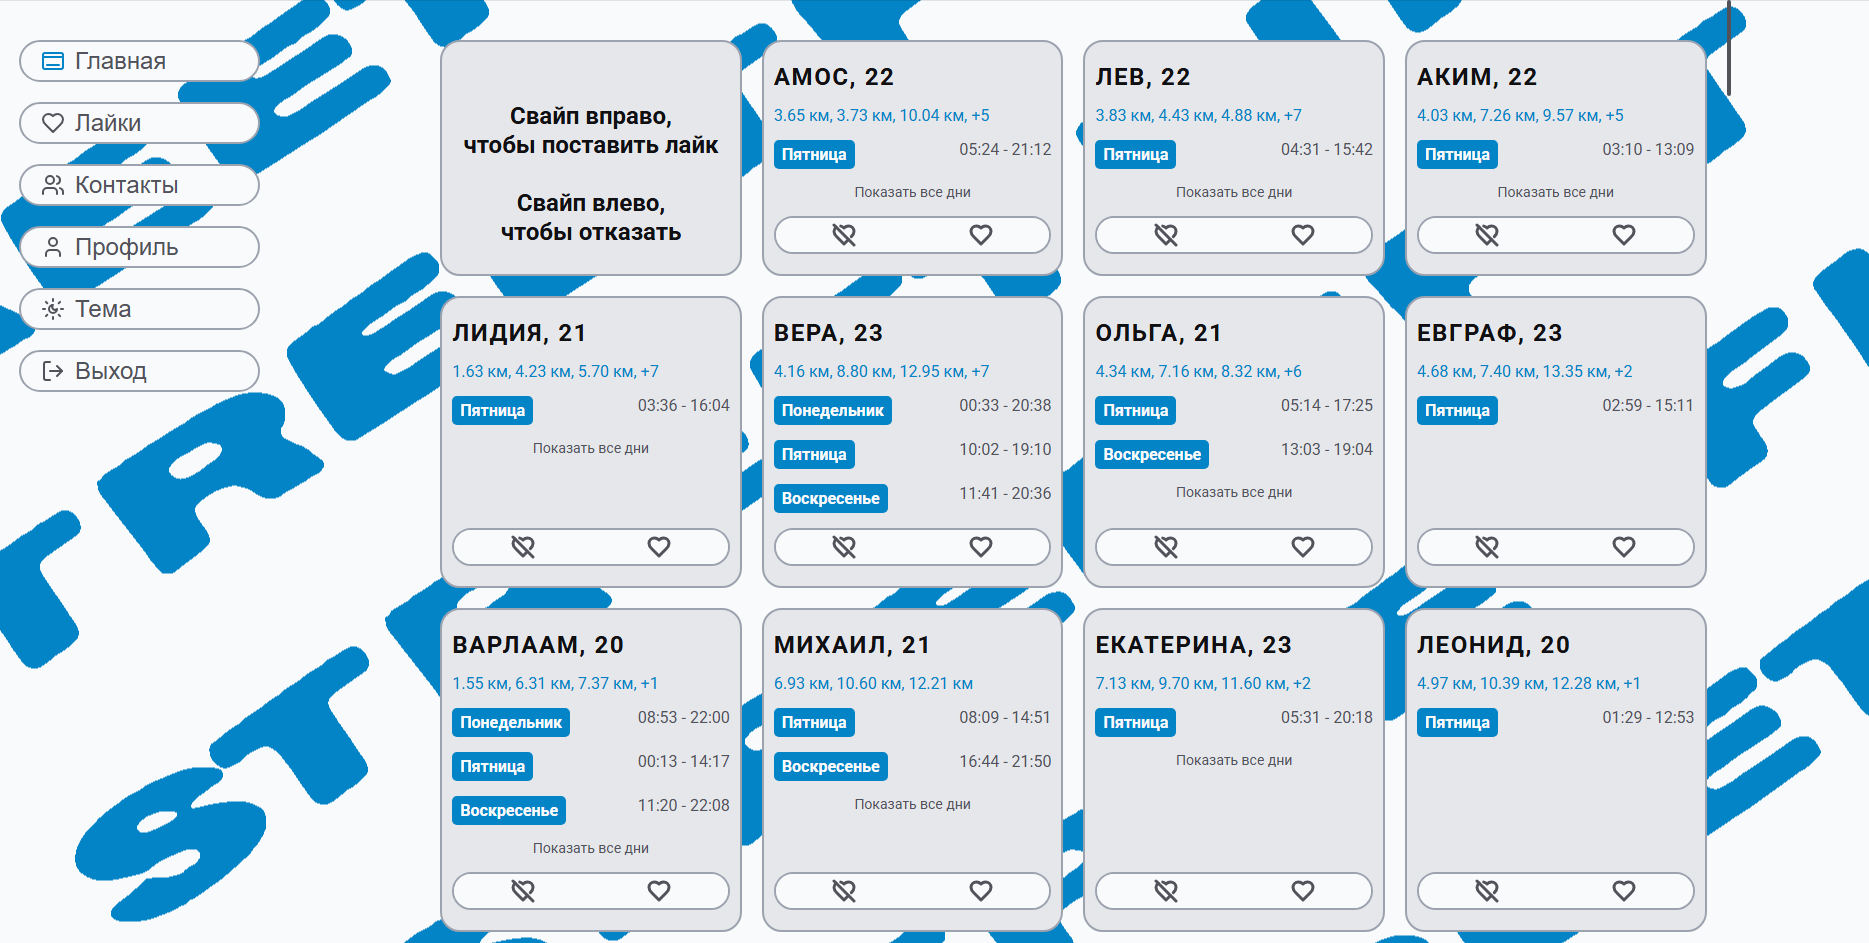
\includegraphics[width=0.8\textwidth]{fig11.png}
	\caption{Пользовательские карточки}
\end{figure}

Пользователь оценивает карточки пользователей, получает их лайки, а в случае мэтча – их контакты.

\begin{figure}[H!]
	\centering
	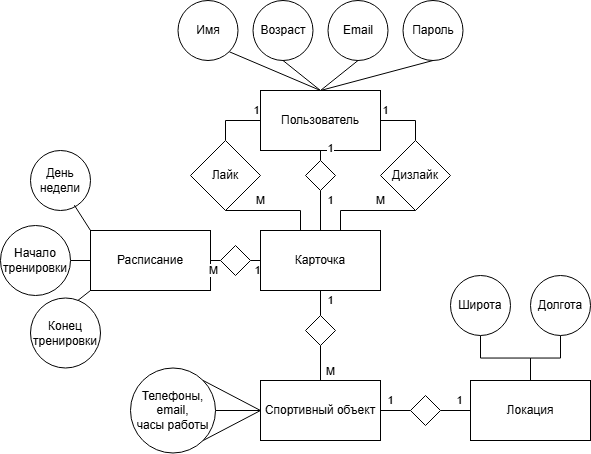
\includegraphics[width=0.8\textwidth]{fig1.png}
	\caption{Карточка пользователя с развернутой картой}
\end{figure}

\newpage
\section*{Заключение}

Разработанное веб-приложение "Streetfit" представляет собой современное решение для поиска
спортивных партнеров, сочетающее инновационные технологии с удобным интерфейсом. Ключевым
достижением работы стала успешная реализация системы взаимного подбора пользователей, что
обеспечивает точную географическую привязку и безопасное установление контактов.

Основные преимущества системы:
\begin{itemize}
	\item Удобный механизм поиска с использованием swipe-интерфейса;
	\item Авторизация пользователей;
	\item Оптимизированная архитектура на основе React и Node.js;
	\item Адаптивный дизайн для мобильных устройств.
\end{itemize}

Ограничения текущей реализации включают зависимость от внешних картографических сервисов и
необходимость ручной модерации контента. Перспективы развития проекта предполагают:
\begin{itemize}
	\item Внедрение машинного обучения для улучшения подбора партнеров;
	\item Расширение интеграции с фитнес-трекерами;
	\item Добавление системы групповых тренировок;
	\item Добавление чата для общения пользователей прямо в приложении.
\end{itemize}

Проект имеет практическую ценность для городских жителей, способствуя популяризации здорового образа жизни и созданию спортивного сообщества.

Ссылка на GitHub репозиторий: https://github.com/Danilb56/open-data
\newpage
\section*{Список литературы}
\begin{enumerate}
	\item React // URL: (дата обращения: 16.04.2024)
	\item React-Router // URL: (дата обращения: 16.04.2024)
	\item JavaScript API Яндекс Карт // URL: (дата обращения: 16.04.2024)
	\item Express // URL: (дата обращения: 16.04.2024)
	\item JWT // URL: (дата обращения: 16.04.2024)
\end{enumerate}
\end{document}
